% !TeX spellcheck = ru_RU
\documentclass[a4paper,12pt]{extarticle}
\usepackage[utf8x]{inputenc}
\usepackage[T1,T2A]{fontenc}
\usepackage[russian]{babel}
\usepackage{hyperref}
\usepackage{indentfirst}
\usepackage{listings}
\usepackage{color}
\usepackage{here}
\usepackage{array}
\usepackage{multirow}
\usepackage{graphicx}

\usepackage{caption}
\renewcommand{\lstlistingname}{Программа} % заголовок листингов кода

\bibliographystyle{ugost2008ls}

\usepackage{listings}
\lstset{ %
extendedchars=\true,
keepspaces=true,
language=C,						% choose the language of the code
basicstyle=\footnotesize,		% the size of the fonts that are used for the code
numbers=left,					% where to put the line-numbers
numberstyle=\footnotesize,		% the size of the fonts that are used for the line-numbers
stepnumber=1,					% the step between two line-numbers. If it is 1 each line will be numbered
numbersep=5pt,					% how far the line-numbers are from the code
backgroundcolor=\color{white},	% choose the background color. You must add \usepackage{color}
showspaces=false				% show spaces adding particular underscores
showstringspaces=false,			% underline spaces within strings
showtabs=false,					% show tabs within strings adding particular underscores
frame=single,           		% adds a frame around the code
tabsize=2,						% sets default tabsize to 2 spaces
captionpos=t,					% sets the caption-position to top
breaklines=true,				% sets automatic line breaking
breakatwhitespace=false,		% sets if automatic breaks should only happen at whitespace
escapeinside={\%*}{*)},			% if you want to add a comment within your code
postbreak=\raisebox{0ex}[0ex][0ex]{\ensuremath{\color{red}\hookrightarrow\space}},
texcl=true,
inputpath=listings,                     % директория с листингами
}

\usepackage[left=2cm,right=2cm,
top=2cm,bottom=2cm,bindingoffset=0cm]{geometry}

%% Нумерация картинок по секциям
\usepackage{chngcntr}
\counterwithin{figure}{section}
\counterwithin{table}{section}

%%Точки нумерации заголовков
\usepackage{titlesec}
\titlelabel{\thetitle.\quad}
\usepackage[dotinlabels]{titletoc}

%% Оформления подписи рисунка
\addto\captionsrussian{\renewcommand{\figurename}{Рисунок}}
\captionsetup[figure]{labelsep = period}

%% Подпись таблицы
\DeclareCaptionFormat{hfillstart}{\hfill#1#2#3\par}
\captionsetup[table]{format=hfillstart,labelsep=newline,justification=centering,skip=-10pt,textfont=bf}

%% Путь к каталогу с рисунками
\graphicspath{{fig/}}

\usepackage{minted}

\begin{document}	% начало документа

% Титульная страница
\begin{titlepage}	% начало титульной страницы

	\begin{center}		% выравнивание по центру

		\large Санкт-Петербургский политехнический университет Петра Великого\\
		\large Институт компьютерных наук и технологий \\
		\large Кафедра компьютерных систем и программных технологий\\[6cm]
		% название института, затем отступ 6см
		
		\huge Телекоммуникационные технологии\\[0.5cm] % название работы, затем отступ 0,5см
		\large Отчет по лабораторной работе №7\\[0.1cm]
		\large Помехоустойчивое кодирование\\[5cm]

	\end{center}


	\begin{flushright} % выравнивание по правому краю
		\begin{minipage}{0.25\textwidth} % врезка в половину ширины текста
			\begin{flushleft} % выровнять её содержимое по левому краю

				\large\textbf{Работу выполнил:}\\
				\large Графов Д.И.\\
				\large {Группа:} 33531/2\\
				
				\large \textbf{Преподаватель:}\\
				\large Богач Н.В.

			\end{flushleft}
		\end{minipage}
	\end{flushright}
	
	\vfill % заполнить всё доступное ниже пространство

	\begin{center}
	\large Санкт-Петербург\\
	\large \the\year % вывести дату
	\end{center} % закончить выравнивание по центру

\thispagestyle{empty} % не нумеровать страницу
\end{titlepage} % конец титульной страницы

\vfill % заполнить всё доступное ниже пространство


% Содержание
\setcounter{page}{2}
% Содержание
\renewcommand\contentsname{\centerline{Содержание}}
\tableofcontents
\newpage




\section{Цель работы}
Изучить воздействие ФНЧ на тестовый сигнал с шумом.

\section{Программа работы}
\begin{itemize}
	\item Сгенерировать гармонический сигнал с шумом и синтезировать ФНЧ.
	\item Получить сигнал во временной и частотной областях до и после фильтрации.
	\item Сделать выводы о воздействии ФНЧ на спектр сигнала.
\end{itemize}

\section{Теоретическая информация}
Аддитивный белый гауссовский шум (АБГШ, англ. AWGN) — вид мешающего воздействия в канале передачи информации. Характеризуется равномерной, то есть одинаковой на всех частотах, спектральной плотностью мощности, нормально распределёнными временными значениями и аддитивным способом воздействия на сигнал. Наиболее распространённый вид шума, используемый для расчёта и моделирования систем радиосвязи. Термин «аддитивный» означает, что данный вид шума суммируется с полезным сигналом и статистически не зависим от сигнала. В противоположность аддитивному, можно указать мультипликативный шум — шум, перемножающийся с сигналом.

\newpage
\section{Ход выполнения работы}
Данная работа выполнялась на языке Python.

В качестве шума был выбран аддитивный белый гауссовский шум с параметрами: 
\begin{itemize}
	\item математическое ожидание: 0;
	\item среднеквадратичное отклонение: 0.5.
\end{itemize}
Затем данный шум был прибавлен к исходному гармоническому сигналу с амплитудой равной 1 и частотой равной 20 Гц.

Далее была осуществлена фильтрация c помощью filtfilt() пакета signal.
Затем были получены графики во временных и частотных областях исходного и отфильтрованного сигнала.

\large {Листинг 1. main.py}
\inputminted[
frame=lines,
framesep=2mm,
baselinestretch=1.2,
fontsize=\footnotesize,
linenos
]{python}{../src/main.py}

\newpage
\large {Результат работы}
\begin{figure}[H]
	\begin{center}
		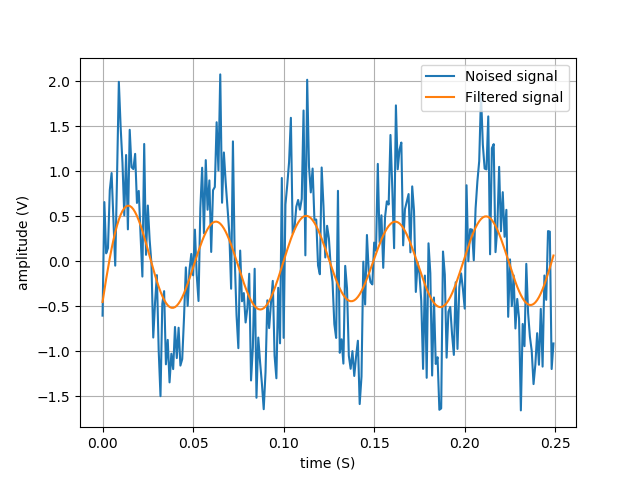
\includegraphics[scale=0.7]{../out/sine_time.png}
		\caption{Синусоидальный сигнал} 
		\label{pic:sine_time} % название для ссылок внутри кода
	\end{center}
\end{figure}

\begin{figure}[H]
	\begin{center}
		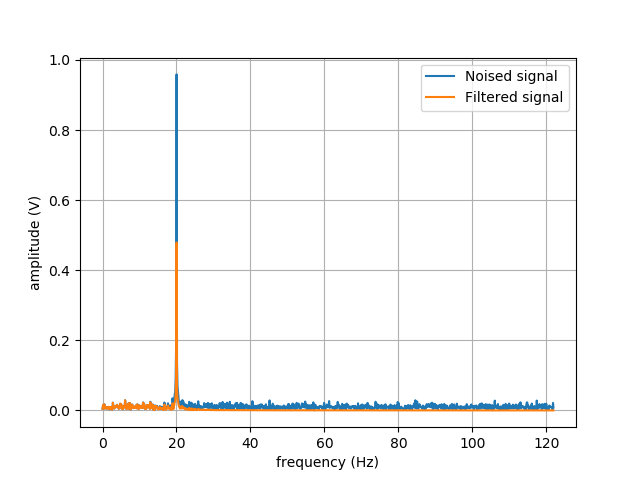
\includegraphics[scale=0.7]{../out/sine_freq.png}
		\caption{Спектр синусоидального сигнала} 
		\label{pic:sine_freq} % название для ссылок внутри кода
	\end{center}
\end{figure}

\newpage
\section{Выводы}
В ходе выполнения работы мной была осуществлена фильтрация гармонического сигнала.

После фильтрации удалось сохранить значимую часть сигнала: была сохранена частота. Однако, в два раза уменьшилась амплитуда.

Спектрограмма показывает относительный успех фильтрации: шумов стало значительно меньше, особенно в области высоких частот.

Непостоянство амплитуды обусловлено остаточным низкочастотным шумом.
\end{document}
